\section{Applications}
\Yaxin{This section is highly incomplete... Each subsection contains some to do list and I'll do more research. } 

For convenience of discussion DMPF applications, we use $\DMPF_{t, N, \GG}$ to denote a DMPF scheme for $t$-point functions with domain $[N]$ and output group $\GG$. 

\begin{table*}
  \caption{Concrete applications of DMPF. }
  \label{tab:app_parameters}
	\begin{tabular}{ccc}
    \toprule
		Concrete application &\makecell{Cost in terms of DMPF\\per correlation/execution}& Typical DMPF parameters \\
    \midrule
		PCG for OLE from Ring-LPN &\makecell{seedsize $\propto$ DMPF.$keysize$\\expand time $\propto$ DMPF.$FullEval()$} & \makecell{$t = 5^2, 16^2, 76^2$\\$N = 2^{20}$}  \\
		PSI-WCA & \makecell{communication $\propto$ DMPF.$keysize$\\client computation $\propto$ DMPF.$Gen()$\\server computation $\propto$ DMPF.$Eval()$} & \makecell{$t = $any\\$N = 2^{128}$}\\
    \bottomrule
	\end{tabular}
\end{table*}

\subsection{PCG for OLE from Ring-$\LPN$}
\Yaxin{TBD: 
\begin{itemize}
  \item Characterize parameters
  \item Show nonregular optimization
  \item Plug in new DMPF and show overall optimization
\end{itemize}}

We begin by briefly introducing the protocol of PCG for OLE from Ring-$\LPN$ assumption, proposed in \cite{cryptoeprint:2022/1035}. 

\paragraph{The PCG protocol for OLE correlation}The hardness assumption we will make use of is a variant of Ring-$\LPN$, called module-$\LPN$ assumption. 
\begin{definition}[Module-$\LPN$]\label{def:module-LPN}
    Let $c\ge 2$ be an integer, $R = \ZZ_p[X]/F(X)$ for a prime $p$ and a deg-$N$ polynomial $F(X)\in \ZZ_p[X]$, and $\mathcal{HW}_{R,t}$ be the uniform distribution over \`weight-$t$\' polynomials in $R$ whose degree is less than $N$ and has at most $t$ nonzero coefficients. 
    %(We write $\mathcal{HW}_t$ when $R$ is clear from the context. )
     For $R=R(\lambda)$, $t=t(\lambda)$ and $m=m(\lambda)$, we say that the module-$\LPN$ problem $R^c$-$\LPN$ is hard if for every nonuniform polynomial-time probabilistic distinguisher $\cA$, it holds that 
    \[
        |\Pr[\cA(\{\vec{a}^{(i)}, \ipd{\vec{a}^{(i)}}{\vec{s}}+\vec{e}^{(i)}\}_{i\in [m]})] - \Pr[\cA(\{\vec{a}^{(i)},\vec{u}^{(i)}\}_{i\in [m]})] \le \mathsf{negl}(\lambda)
    \]
    where the probabilities are taken over the randomness of $\cA$, random samples $\vec{a}^{(1)},\cdots, \vec{a}^{(m)}\leftarrow R^{c-1}$, $\vec{u}^{(1)},\cdots, \vec{u}^{(m)}\leftarrow R$, $\vec{s}\leftarrow \cHW_{R,t}^{c-1}$, and $\vec{e}^{(1)},\cdots, \vec{e}^{(m)}\leftarrow \cHW_{R,t}$. 

    When we only consider $m=1$, each $R^c$-$\LPN$ instance $ \ipd{\vec{a}}{\vec{s}}+\vec{e}$ can be restated as $\ipd{\vec{a'}}{\vec{e'}}$ where $\vec{a'}=1||\vec{a}$ and $\vec{e'}\leftarrow \cHW_{R,t}^c$. 
\end{definition}

The PCG protocol in \cite{cryptoeprint:2022/1035} generates seed for the OLE correlation $(x_0,x_1,z_0,z_1)\in R^4$ such that $x_0+x_1 = z_0\cdot z_1$. The idea is to first set $z_b = \ipd{\vec{a}}{\vec{e_b}}$ (an $R^c$-$\LPN$ instance with public $\vec{a}$ and $\vec{e_b}\leftarrow \cHW_{R,t}^c$). Basing on the fact that $\ipd{\vec{a}}{ \vec{e_0}}\cdot \ipd{\vec{a}}{\vec{e_1}} = \ipd{\vec{a}\otimes \vec{a}}{\vec{e_0}\otimes \vec{e_1}}$, the next step is to additively share the tensor product $\vec{e_1}\otimes \vec{e_1}$ and each party can compute an additive share of $z_0\cdot z_1$. Note that the tensor product $\vec{e_0}\otimes\vec{e_1}$ consists of $c^2$ entries, each being an deg-$2N$ polynomial with at most $t^2$ nonzero coefficients. Therefore it can be shared by invoking $\DMPF_{t^2, 2N, \mathbb{Z}_p}$ for $c^2$ times.

One can compute the seed size and expanding time of this PCG protocol as follows: 
\begin{itemize}
    \item The seed size is $ct(\log N+\log p)$ bits for specifying $\vec{e_b}$ plus the $c^2\times $keysize of $\DMPF$. 
    \item The expanding time is $c^2N$ multiplications in $R$ plus $c^2\times$full-domain evaluation time of $\DMPF$. 
\end{itemize}

\begin{remark}\label{rem:use_reducible_ring}
    Note that the above PCG protocol generates seed for OLE correlation over ring $R$. One can immediately convert an OLE correlation over ring $R$ to $N$ OLE correlations over $\ZZ_p$ if the polynomial $F(X)$ splits into $N$ distinct linear factors modulo $p$. Therefore we mostly consider reducible $F$ of such form. 
\end{remark}

A previous optimization is to substitute $\cHW_{R,t}$ with regular weight-$t$ polynomials denoted as regular-$\cHW_{R,t}$. Each regular weight-$t$ polynomial $e$ contains exactly one nonzero coefficient $e_j$ in the range of degree $[j\cdot (N/t), (j+1)\cdot (N/t)-1]$ for $j=0,\cdots t-1$. When multiplying two regular weight-$t$ polynomials $e$ and $f$, $e_i\cdot f_j$ contributes to a coefficient in the range of degree $[(i+j)\cdot (2N/t), (i+j+2)\cdot (2N/t)-2]$. Therefore the deg-$2N$ polynomial $e\cdot f$ can be shared by invoking $\{\DMPF_{k, 2N/t, \mathbb{Z}_p}\}_{k=1,2,\cdots,t-1,t,t-1,\cdots, 2,1}$, which cuts down the domain size compared to the original design. 

The previous literature uses sum of DPFs to achieve DMPF in either the original design with nonregular noise or the optimized design with regular noise. It indicates using batch code to achieve DMPF as another optimization but not in the clear. We'll analyze the cost of this PCG protocol when 
\begin{itemize}
    \item[(1)]with regular noise and each multiplication of sparse polynomials is shared by 2 sets of $\{\DMPF_{k, 2N/t, \mathbb{Z}_p}\}_{1\le k\le t-1}$ and $\DMPF_{t, 2N/t, \mathbb{Z}_p}$;
    \item[(2)]with nonregular noise and each multiplication of sparse polynomials is shared by $\DMPF_{t^2, 2N, \mathbb{Z}_p}$. 
\end{itemize}
We'll instantiate $\DMPF$ in different ways as listed in \cref{tab:formulas_DMPF_comparison}. 
\begin{table*}
    \caption{Comparison among different choices of noise distribution in module-LPN assumption, and their seed size and expanding time using different DMPF constructions. The }
	\label{tab:LPN_error_distribution}
		\begin{tabular}{cccc}
            \toprule
			$\DMPF$ scheme & Noise type & Total share size & Total $\FullEval$ time \\
            \midrule
			 & regular & $c^2t^2\lambda\log(2N/t)$ & \makecell{$2c^2tN\times$PRG (DPF); \\ ${4c^2N}\times $PRG$+4c^2\hat{g}N\times \mathbb{F}_{2^{2^{\lambda+2}}}$-MUL (OKVS-DMPF)}\\
			 & nonregular & $c^2t^2\lambda\log(2N)$ &\makecell{ $2c^2t^2N\times$PRG (DPF); \\${2c^2N}\times$PRG$+2c^2\hat{g}N\times\mathbb{F}_{2^{\lambda+2}}$-MUL (OKVS-DMPF)}\\
            \bottomrule
		\end{tabular}
\end{table*}

Next we plug in concrete parameters and evaluate the performance of different $\DMPF$ schemes under different PCG parameter settings. 

Define the number of noisy coordinate $w:=ct$. We set $(\lambda, c, N, w)$ such that the best attack requires at least $2^\lambda$ arithmetic operations over field $\FF_p$ of size approximately $2^{128}$. According to \cite{cryptoeprint:2022/1035}, for $R$ from irreducible $F$, we lowerbound the number of arithmetic operations by $N\cdot (c\cdot \frac{N}{N-1})^w\approx N\cdot c^w$. For $R$ from reducible $F$, we lowerbound the number of arithmetic operations by $2^i\cdot c^{w_i}$ \Yaxin{(to be checked)}, where $i:=\mathop{\arg\min}\limits_{1\le i\le \log N}\left((\frac{c\cdot 2^i}{(c-1)\cdot 2^i-1})^{w_i}\cdot 2^i\right)$ and $w_i:=c(c-1)\cdot 2^i\left(1-(1-\frac{1}{(c-1)2^i})^{w/c}\right)$. \Yaxin{(to be checked) In the end we round $w$ such that $t=w/c$ is an integer. }


\Yaxin{\textbf{Does entropy gain leads to significant efficiency improvement? }Notice that under the same $N,c$ and $t$, $E_2>E_1$ and $E_2-E_1 \approx ct\log \mathrm{e}$. Now let's suppose $c$ and $N$ are always fixed and $t_1, t_2$ are the choices of $t$ for the first and second distribution such that they reach the same entropy. When $N\gg t$ we have the relation $\frac{t_1}{t_2} \approx (1+1/\log N)$, which is not a big difference. \\}

From \cref{tab:LPN_error_distribution} we can see that the noise distribution $regular$-$\mathcal{HW}_t$ should be preferred if we instantiate DMPF in PCG for OLE through sum of DPF's, while $\mathcal{HW}$ should be preferred if we instantiate DMPF through the big-state, batch-code or OKVS-DMPF. 

Now let's compare the seed size and expand time of PCG with different DMPF instantiations in \cref{fig:detailed_PCG}, where the naive (DPF) one has regular noise distribution. For extremely small $t$ ($t<8$), the big-state DMPF yields the best expand time, at the expense of slightly larger seed size. For $t\ge 8$ the seed size of the big-state DMPF becomes incomparable to others while the expand time of the big-state DMPF grows with $t$ and exceeds that of the naive DPF construction when $t$ is around 130, which is larger than the typical parameters. 

The expand time of the batch-code or OKVS-DMPF doesn't grow with $t$, and the expand time of OKVS-DMPF is about $0.5\times $ that of the batch-code-DMPF. However the seed size yielded by OKVS-DMPF is usually larger than the batch-code-DMPF. When $t$ is as small as 8, the seed size yielded by OKVS-DMPF is only slightly larger, but when $t$ grows to the largest typical parameter 76, the OKVS-DMPF is about $\times 2$ of the seed size of the batch-code-DMPF. 



\Yaxin{Previous calculation as a reference: } choosing the big-state DMPF for $t<8$ and the OKVS-DMPF for $t\ge 8$ gives at least $\times 2$ acceleration on expand time over other choices with sacrifice on the keysize. There is a tradeoff between the batch-code and OKVS-DMPF in that the OKVS-DMPF always provides a $\sim\times 2$ acceleration on expand time, but a loss in seed size that when $t$ is large it may blow up the seed size to $\sim \times 2$ that of the batch-code-DMPF. 

\begin{figure}[H]
	\centering
	\subfigure{
		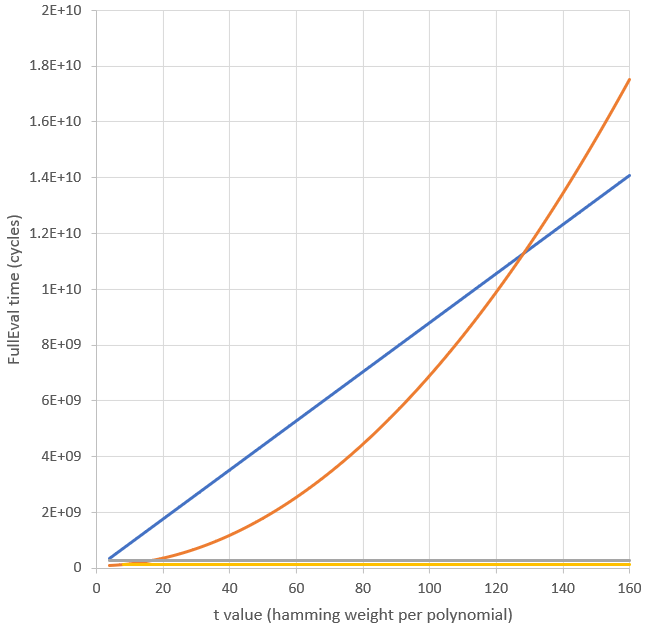
\includegraphics[scale = 0.4]{figures/FullEval_time_PCG.png}
	}
	\subfigure{
		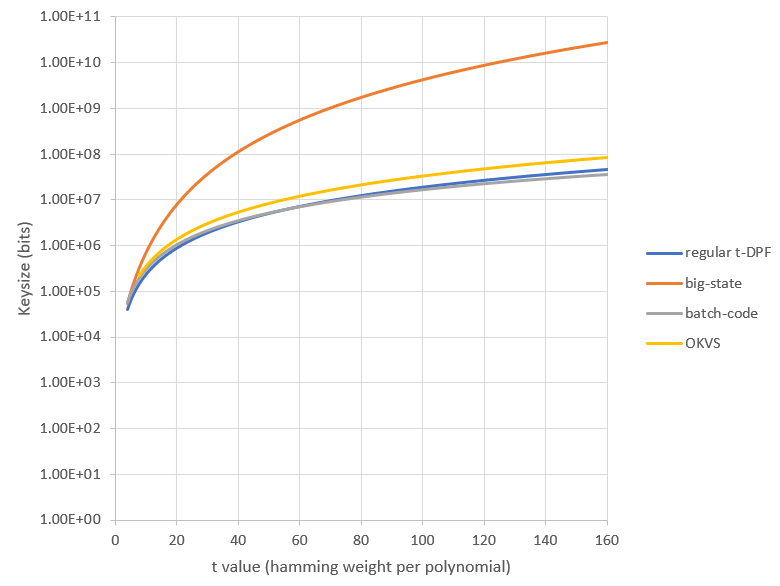
\includegraphics[scale = 0.4]{figures/keysize_PCG.png}
	}
	\caption{Full-domain Evaluation time and keysize of DMPF used in PCG for OLE\cite{cryptoeprint:2022/1035} using four different DMPF constructions. Consider the security parameter $\lambda=128$, the domain size $N = 2^{20}$ and various noise weights per $R$-element, from 4 to 160 (the typical weights per $R$-element in \cite{cryptoeprint:2022/1035} are 5, 16 and 76). To obtain little failure probability, the OKVS-DMPF is only applicable for $t\ge 8$ as considered in \cite{cryptoeprint:2022/320}. PRG evaluation is modeled as two AES evaluations with AES evaluation time $1.3$ cycles per byte. Field multiplications in OKVS-DMPF approach $0.3$ cycles per byte \cite{cryptoeprint:2017/168} for the corresponding field. The actual expand time and seed size of PCG is $\sim \times c^2$ of that the FullEval time and key size of DMPF, where $c$ is the compression factor. }
	\label{fig:detailed_PCG}
\end{figure}

\subsection{PSI-WCA}
\Yaxin{TBD: 
\begin{itemize}
  \item plug in new DMPF and analyze advantage interval
  \item plug in distributed gen
\end{itemize}}
\Yaxin{Previous calculation as a reference: }A short conclusion is using big-state DMPF for $t<64$ and the OKVS-DMPF for $t\ge 64$ gives at $\sim \times 2$ faster Eval() time and faster Gen() time compared to the naive and batch-code construction. The keysize ($\propto$ communication complexity) of our choice is usually smaller than the batch-code DMPF and slightly larger than the naive construction. 
\subsection{Security analysis}
\subsection{Heavy-hitters}
private heavy-hitter\\
or parallel ORAM?